\documentclass{article}

\usepackage[utf8]{inputenc} % Підтримка UTF-8
\usepackage[ukrainian]{babel} % Підтримка української мови
\usepackage[ukrainian=nohyphenation]{hyphsubst} 
\usepackage{booktabs}
\usepackage[T2A]{fontenc} % Кодова таблиця для кирилиці
\usepackage{amsmath, amsfonts} % Для математики, якщо потрібно
\usepackage[a4paper, left=3cm, right=1.5cm, top=2cm, bottom=2cm]{geometry}
\usepackage{fancyhdr}        % Пакет для налаштування колонтитулів
\usepackage{hyperref}        % Для створення посилань
\usepackage{listings}          % Пакет для вставки коду
\usepackage{graphicx}
\usepackage{csvsimple}
\usepackage{parskip}
\usepackage{csquotes}
\usepackage{pgfplotstable}
\usepackage{xcolor}      % For custom colors

\pagestyle{fancy}            % Встановлюємо fancy стиль для колонтитулів
\fancyhf{}                   % Очищуємо всі колонтитули
% Встановлюємо посилання на зміст у лівий верхній кут
\fancyhead[L]{\hyperlink{mytarget}{Зміст}}  % Посилання на зміст
% Встановлюємо нумерацію сторінок у правий верхній кут
\fancyhead[R]{\thepage}
% Прибираємо колонтитули з першої сторінки
\thispagestyle{plain}
% Прибираємо колонтитули для першої сторінки
\fancypagestyle{plain}{
    \fancyhf{}  % Очищуємо колонтитули
    \renewcommand{\headrulewidth}{0pt}  % Вимикаємо лінію колонтитулів
}
\hypersetup{
    colorlinks=true,        % Enable colored links
    linkcolor=red!50!black,      % Color for internal links
    citecolor=red!50!black,      % Color for citations
    filecolor=red!50!black,      % Color for file links
    urlcolor=red!50!black        % Color for external URLs
}

\graphicspath{{../../../}}

\setlength{\emergencystretch}{3cm}

\usepackage{subfiles}

\begin{document}
% Титульна сторінка
\newpage 
\begin{center}
    \LargeНАЦІОНАЛЬНИЙ ТЕХНІЧНИЙ УНІВЕРСИТЕТ УКРАЇНИ\\
    \Large«КИЇВСЬКИЙ ПОЛІТЕХНІЧНИЙ ІНСТИТУТ\\
    \LargeІМЕНІ ІГОРЯ СІКОРСЬКОГО»\\
    \vspace{1cm}
    Факультет прикладної математики\\
    Кафедра прикладної математики\\
    \vspace{3cm}
    \textbf{Звіт}\\
    \vspace{0.5cm}
    із лабораторної роботи №1\\
    із дисципліни «Аналіз даних»\\
    \vspace{1cm}
    на тему\\
    \textit{Розвідковий аналіз даних}\\
    \vspace{1.5cm}
    \textbf{Команда № 9}\\
    \vspace{2cm}
    \begin{tabbing}
        Виконали: \hspace{10cm} \= Керівник:\\
        студенти групи КМ-23: \> \textit{Тавров Д.Ю.}\\
        \textit{Баранівська В.О.} \> \textit{Доцент,}\\
        \textit{Корсун Є. В.} \> \textit{канд. тех.-наук}.\\
        \textit{Хмарук О. Ю.} \> \\
        \textit{Літковський А.С.} \>\\
        \textit{Кудін Н. А.} \> \\
    \end{tabbing}
    \vspace{3cm}
    \largeКиїв — 2025\\
\end{center}

% Створюємо зміст
\newpage
\hypertarget{mytarget}{} % Якір на сторінці 5
\tableofcontents
\newpage

\section{Вступ}
\subsection{Мета}
Протягом останнього десятиліття, якість повітря у світі суттєво погіршується. Завдяки вимірам та аналізу вчених, можна нагаматися покращити або ж мінімізувати ті, чи інші шкідливі викиди газів і не тільки. 

Низка соціально-наукових дослдіжень показують, що стрімке погіршення якості повітря все ще залишається в густо населених регіонах. Тому, щоб провести аналіз даної галузі, було проведено пошук набору даних в країнах Азії. 

В ході дослідження ресурсів зі збору даних у цьому напрямі, було вирішено дослідити якість повітря Тайваню. Уряд провінції намагається контролювати та покращувати якість повітря. Тому 17 грудня 2017 року була введена  реформа Air Pollution Control Action Plan. \footnote{\href{https://e-info.org.tw/node/209138}{Покликання на статтю про запровадження реформи 3 2017 по 2040 роки}}.

\begin{center}
    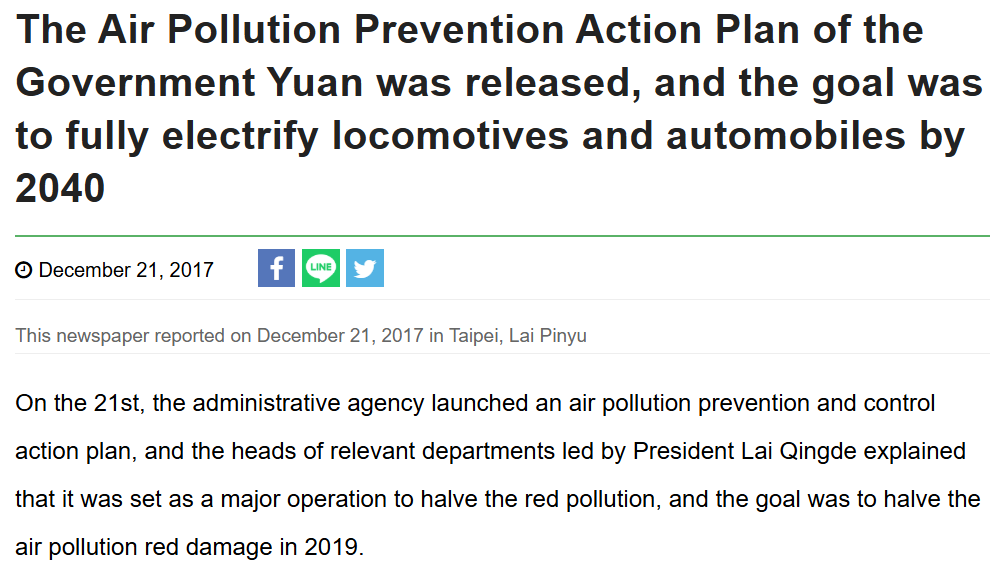
\includegraphics[height=3in]{notes/media/air_quality_reform_news.png}\\
    \textit{Вирізка зі статті про початок реформи}
\end{center}

\subsection{Постановка задачі}
З огляду на мету та досліджувану галузь, було поставлено такі питання: 

\begin{enumerate}
    \item Чи впливає швидкість вітру (windspeed) на концентрацію частинок PM2.5 і PM10?
    \item  Чи існує кореляція між рівнем забруднення повітря (AQI) і типом головного забруднювача (pollutant) в різних районах?
    \item Як зміни в концентрації озону (O3) впливають на загальний рівень забруднення повітря (AQI)?
    \item Які регіони (county) мають найвищий середній рівень забруднення повітря (AQI) протягом року?
    \item Як змінюється якість повітря (status) протягом доби в різних районах?
    \item Як змінюється концентрація PM2.5 і PM10 в залежності від швидкості вітру (windspeed) і напрямку вітру (winddirec) в різних регіонах?
    \item Як змінився загальний рівень забруднення по регіонам після початку реформи? 
    \item Чи існує залежність між початком реформ та показниками забруднення? 
    \item Як змінюється якість повітря залежно від станції виміру у містах?
\end{enumerate}

    
\newpage

\subfile{main_part.tex}

\pagebreak

\subfile{eda.tex}

\pagebreak

\newpage
\section{ВИСНОВОК}
В результаті виконання лабораторної роботи було проведено розвідковий аналіз результатів виміру якості повітрю регіонів Тайваню з 2016 року по 2024. 

На жаль не вдалось відповісти на деякі поставлені питання, через значну кількість відсутніх даних у стовпці $'pollutant'$, а саме не дали відповідь на: 
\begin{enumerate}
    
    \item  Чи існує кореляція між рівнем забруднення повітря (AQI) і типом головного забруднювача (pollutant) в різних районах?
    
\end{enumerate}
Відповіді на ці питання сподіваємось уряд Тайваню, зможе в скорому часі оприлюднити.


%На основі аналізу залежності викидів та регіонів, можна зробити наступні висновки: 


Гістограми, побудовані на основі видобутих даних, повинні демонструвати характерну залежність тих чи інших речовин у повітрі відповідно до регіону, часу доби та швидкості вітру.

Отже, після розвідкового аналізу та побудови графіків, можна дати відповіді на наступні питання:
\begin{enumerate}
    \item Чи впливає швидкість вітру (windspeed) на концентрацію частинок PM2.5 і PM10?
    
    \item Як зміни в концентрації  ($O_3$)  та $SO_2$ впливають на загальний рівень забруднення повітря (AQI)?
    
    \item Як змінюється якість повітря (status) протягом доби в різних районах?
    
    \item Які регіони (county) мають найвищий середній рівень забруднення повітря (AQI) протягом року?
     
    \item Як змінився загальний рівень забруднення по регіонам після початку реформи?
    
    \item Чи існує залежність між початком реформ та показниками забруднення?
    
    Після побудови низки гарфіків, було відмічено, що після реформи суттєво змінився лише показник концентрації $S0_2$. Всі ініші показники, не зазнали суттєвих змін.
    
    \item Як змінюється якість повітря залежно від станції виміру у містах?
    
\end{enumerate}


\newpage
\section{Використані джерела}
\begin{enumerate}
    \item Exploratory Data Analysis with R. Home | Bookdown. 
    
    URL:  \href{https://bookdown.org/rdpeng/exdata/}{https://bookdown.org/rdpeng/exdata/}
    
    \item Exploratory Data Analysis | R for Data Science. Welcome | R for Data Science.
    
    URL: \href{https://r4ds.had.co.nz/index.html}{https://r4ds.had.co.nz/index.html}
    \item The R Graph Gallery – Help and inspiration for R charts. The R Graph Gallery. 
    
    URL: \href{ https://r-graph-gallery.com/}{ https://r-graph-gallery.com/ }
\end{enumerate}

\end{document}